\lecture{3}{lun 01 mag 2023 17:10}{Sistema dinamico e moti}
	\lablsection{Sistema dinamico}
	\begin{figure}[H]
		\centering
			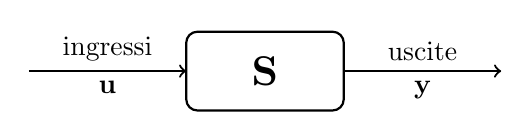
\begin{tikzpicture}[thick]
				\draw[<-] (3,0) -- (2,0)node[below]{$ \textbf{y} $} node[above]{uscite}-- (1,0);
				\draw[rounded corners] (1,.5) rectangle (-1,-0.5); 
				\draw (0,0) node[scale=1.5]{\textbf{S}};
				\draw[->] (-3,0) --(-2,0)node[below]{$ \textbf{u} $}node[above]{ingressi} -- (-1,0);
			\end{tikzpicture}
                        \end{figure}
			%			\includegraphics[width=0.9\linewidth]{"Images/sistemadinamico.png"}
			Ingresso: influenza il sistema\\
			Uscita: obiettivo del problema: vogliamo che tenda ad un riferimento ($ y^0 $)\\
	\nota{La relazione tra $ u $ e $ y $ è di causa effetto.}
	\begin{itemize}
		\item Occorre conoscere le equazioni differenziali
		\item Per risolverlo ci servono gli ingressi istante per istante
		\item Servono le condizioni iniziali
	\end{itemize}
	\lablsubsection{Ordine del sistema}
	Il numero di condizioni iniziali per determinare le uscite, noti gli ingressi istante per istante, è detto \emph{ordine del sistema} $ n $.
	\lablsubsection{Variabili di stato}
	Le $ n $ \emph{variabili di stato} si indicano come:
	\begin{figure}[H]
		\begin{minipage}{.4\textwidth}
			\centering
			\begin{equation*}
				\boxed{x_1,x_2,\dots,x_n}
			\end{equation*}
		\end{minipage}
		\begin{minipage}{.4\textwidth}
			\centering
			\begin{itemize}
				\item $ n $: numero variabili di stato
				\item $ m $: numero ingressi
				\item $ p $: numero uscite
			\end{itemize}
		\end{minipage}
	\end{figure}
	
	\subsubsection{Sistema dinamico in spazio di stato}
	\begin{align*}
		\dot{x}_1 &= f_1(x_1,x_2,\dots,x_n,u_1,u_2,\dots,u_m)\\
		\vdots &\\
		\dot x_n &= f_n(x_1,x_2,\dots,x_n,u_1,u_2,\dots,u_m)
	\end{align*}
	
	\subsubsection{Trasformazione uscita}
	\begin{align*}
		\dot y_1 &= g_1(x_1,x_2,\dots,x_n,u_1,u_2,\dots,u_m)\\
		\vdots &\\
		\dot y_p &= g_p(x_1,x_2,\dots,x_n,u_1,u_2,\dots,u_m)
	\end{align*}
	\lablsubsection{Notazione vettoriale}
	\begin{figure}[H]
		\centering
		\begin{minipage}{0.3\textwidth}
			\centering
			$\underline{x}(t) = \begin{pmatrix} 	x_1 \\ \dots \\	x_n	\end{pmatrix}$
		\end{minipage}
		\begin{minipage}{0.3\textwidth}
			\centering
			$\underline{y}(t) = \begin{pmatrix} 	y_1 \\ \dots \\	y_p	\end{pmatrix}$
		\end{minipage}
		\begin{minipage}{0.3\textwidth}
			\centering
			$\underline{u}(t) = \begin{pmatrix}u_1 \\ \dots \\ u_m\end{pmatrix}$
		\end{minipage}
	\end{figure}
	\begin{figure}[H]
		\centering
		\begin{minipage}{0.4\textwidth}
			\centering
			$f(\underline{x},\underline{u}) = \begin{pmatrix} 	f_1(\underline{x},\underline{u}) \\ \dots \\ f_n(\underline{x},\underline{u})	\end{pmatrix}$
		\end{minipage}
		\begin{minipage}{0.4\textwidth}
			\centering
			$g(\underline{x},\underline{u}) = \begin{pmatrix} 	g_1(\underline{x},\underline{u}) \\ \dots \\ g_p()\underline{x},\underline{u}	\end{pmatrix}$
		\end{minipage}
	\end{figure}
	con $ \vec{x} \in \R^n $, $ \vec{y} \in \R^p $, $ \vec{u} \in \R^m $, $ f \in \R^{n\times m} $ e $ g \in\R^{n\times m} $.\\
	Osservazione: I sistemi considerati sono \emph{tempo-invarianti}, la scelta dell'asse temporale è fatta ponendo $ t_0 =  0$
	\lablsubsection{Classificazione dei sistemi}
	\begin{itemize}
		\item Sistemi \emph{lineari} o \emph{non lineari}
		\item Sistemi "\emph{SISO}" (Single-Input-Single-Output) con $ n = p = 1 $ oppure "\emph{MIMO}" (Multi-Input-Multi-Output)
		\item Sistemi \emph{strettamente propri} (quando $ g $ non dipende da $ u $) e \emph{propri} (quando $ g $ invece dipende da $ u $)
	\end{itemize}
	\subsubsection{Esempi di sistemi in spazio di stato}
	\begin{itemize}
		\item \textbf{Resistore}: $ y = i $, $ u = \text{V} $ $ \to y = \frac{1}{R}u $
		\item \textbf{Induttore}: $ x_1 = 1, u = \text{V}, y = x_1 \to \begin{cases}
			\dot{x}_1 = \frac{1}{L} u \\
			y = x_1
		\end{cases}$
		\item \textbf{Massa}: $ x_1 = p, x_2 = \text{V}, u = \text{F} \to \begin{cases}
			\dot{x}_1 = x_2\\
			\dot{x}_1 = \frac{1}{M}u\\
			y = x_1
		\end{cases}$	
		\item \textbf{Oscillatore armonico}: $ x_1 = p, x_2=\omega, u = \tau\to\begin{cases}
			\dot{x}_1=x_2\\
			\dot{x}_1 = \frac{1}{M}(-Kx_1-\sigma x_2 + u)\\
			y = x_1
		\end{cases} $
		
		\item \textbf{Pendolo}: $ x_1 =h,y=x_1,u=q_i \to\begin{cases}
			\dot{x}_1 = x_2\\
			\dot{x}_1 = -\frac{g}{l} \sin(x_1) + \frac{1}{Ml^2} u\\
			y = x_1
		\end{cases}$
		
		\item \textbf{Serbatoio con valvola}: $ x_1 = h, y = x_1,u=q_1\to \begin{cases}
			\dot{x}_1 = \frac{1}{A_s}u - k\frac{A_v}{A_s}\sqrt{x_1}\\
			y = x_1
		\end{cases} $
	\end{itemize}
	I sistemi si distinguono in non lineari e lineari.
	\lablsubsection{Sistemi lineari}
	I sistemi lineari sono composto dalle \emph{equazioni di stato} che possono essere generalizzate come segue:
	\begin{equation*}
		\begin{cases}
			\dot{x}_1 = a_{11}x_1+a_{12}x_2+\dots+a_{1n}x_n+b_{11}u_1 + \dots+b_{1m}u_m\\
			\dots\\
			\dot{x}_n = a_{n1}x_1+a_{n2}x_2+\dots+a_{nn}x_n+b_{n1}u_1 + \dots+b_{nm}u_m\\
		\end{cases}
	\end{equation*}
	dalle trasformazioni di uscita:
	\begin{equation*}
		\begin{cases}
			y_1 = c_{11}x_1+c_{12}x_2+\dots+c_{1n}x_n+d_{11}u_1 + \dots+d_{1m}u_m\\
			\dots\\
			y_p = c_{p1}x_1+c_{p2}x_2+\dots+c_{pn}x_n+d_{p1}u_1 + \dots+d_{pm}u_m\\
		\end{cases}
	\end{equation*}
	Posso ridurre i due sistemi di equazioni lineari usando quattro matrici:
	\begin{figure}[H]
		\centering
		\begin{minipage}{.5\textwidth}
			\centering
			\[
			A = \begin{bmatrix}
				a_{11} & a_{12} & a_{13} & \dots & a_{1n} \\
				a_{21} & a_{22} & a_{23} & \dots & a_{2n} \\
				\vdots & \vdots & \vdots & \ddots & \vdots \\
				a_{n1} & a_{n2} & a_{n3} & \dots & a_{nn}
			\end{bmatrix}
			\]
		\end{minipage}%
		\begin{minipage}{.5\textwidth}
			\centering
			\[
			B = \begin{bmatrix}
				b_{11} & b_{12} & b_{13} & \dots & b_{1m} \\
				b_{21} & b_{22} & b_{23} & \dots & b_{2m} \\
				\vdots & \vdots & \vdots & \ddots & \vdots \\
				b_{n1} & b_{n2} & b_{n3} & \dots & b_{nm}
			\end{bmatrix}
			\]
		\end{minipage}
		
		\vspace{.1cm}
		
		\begin{minipage}{.5\textwidth}
			\centering
			\[
			C = \begin{bmatrix}
				c_{11} & c_{12} & c_{13} & \dots & c_{1p} \\
				c_{21} & c_{22} & c_{23} & \dots & c_{2p} \\
				\vdots & \vdots & \vdots & \ddots & \vdots \\
				c_{n1} & c_{n2} & c_{n3} & \dots & c_{np}
			\end{bmatrix}
			\]
		\end{minipage}%
		\begin{minipage}{.5\textwidth}
			\centering
			\[
			D = \begin{bmatrix}
				d_{11} & d_{12} & d_{13} & \dots & d_{1m} \\
				d_{21} & d_{22} & d_{23} & \dots & d_{2m} \\
				\vdots & \vdots & \vdots & \ddots & \vdots \\
				d_{n1} & d_{n2} & d_{n3} & \dots & d_{nm}
			\end{bmatrix}
			\]
		\end{minipage}
	\end{figure}
	Dunque il problema può essere riassunto nel seguente sistema:
	\begin{equation*}
		\begin{cases}
			\underline{\dot{x}} = \hat{A}\underline{x}+ \hat{B}\underline{u}\\
			\underline{y} = \hat{C}\underline{x}+\hat{D}\underline{u}
		\end{cases}
	\end{equation*}
	\lablsubsection{Movimento (moto)}
	Il moto dello stato è l'evoluzione nel tempo del vettore di stato date le condizioni iniziali e gli andamenti degli ingressi. Analoga è la definizione di moto dell'uscita. In generale, le equazioni del moto dello stato sono utilizzate per descrivere come i segnali di ingresso influenzano lo stato del sistema e come lo stato del sistema cambia nel tempo. Possono anche essere utilizzate per calcolare le risposte del sistema a determinate perturbazioni o a segnali di ingresso specifici.\\
	Per i sistemi lineari distinguiamo due termini di moto:
	\begin{enumerate}
		\item \textbf{Moto libero}: dipende dalle condizioni iniziali
		\item \textbf{Moto forzato}: dipende dagli ingressi
	\end{enumerate}
	In generale il moto è la somma di una componente libera e di una forzata.
	\begin{figure}[H]
		\begin{minipage}[t]{0.5\textwidth}
			\subsubsection{Moto libero}
			\begin{align*}
				x_l(t) = &e^{at}x_0\\
				y_l(t) = C&e^{at}x_0
			\end{align*}
		\end{minipage}
		\begin{minipage}[t]{0.5\textwidth}
			\subsubsection{Moto forzato}
			\begin{align*}
				x_f(t) = &\int^t_0 e^{a(t-\tau)}bu(\tau)\,d\tau\\
				y_f(t) =C&\int^t_0 e^{a(t-\tau)}bu(\tau)\,d\tau
			\end{align*}
		\end{minipage}
	\end{figure}
	
	\lablsubsection{Equilibri (moti costanti)}
	Supponiamo che  $u = \overline{u}$ , $\overline{u}$ costante.\\
	L'equilibrio corrispondente a $\overline{u}$ è il moto  costante di stato e uscita. Andando a sostituire nelle varie equazioni possiamo dedurre che:
	\[    \dot{x} = 0 \]
	\[\dot{x} = f(x,u) \to f(\overline{x},\overline{u} = 0\]
	\[\overline{x} : \text{Stati di equilibrio}\]
	\[\overline{y} = g(\overline{x},\overline{u})\]

%%% Local Variables:
%%% mode: latex
%%% TeX-master: "master"
%%% End:
